\documentclass[12pt, titlepage]{article}

\usepackage{amsmath, mathtools}
\usepackage{siunitx}
\usepackage{fullpage}
% \usepackage[round]{natbib}
\usepackage[numbers,square]{natbib}
\usepackage{multirow}
\usepackage{booktabs}
\usepackage{tabularx}
\usepackage{graphicx}
\usepackage{float}
\usepackage{hyperref}
\hypersetup{
    colorlinks,
    citecolor=blue,
    filecolor=black,
    linkcolor=red,
    urlcolor=blue
}

%% Comments

\usepackage{color}

\newif\ifcomments\commentstrue %displays comments
%\newif\ifcomments\commentsfalse %so that comments do not display

\ifcomments
\newcommand{\authornote}[3]{\textcolor{#1}{[#3 ---#2]}}
\newcommand{\todo}[1]{\textcolor{red}{[TODO: #1]}}
\else
\newcommand{\authornote}[3]{}
\newcommand{\todo}[1]{}
\fi

\newcommand{\wss}[1]{\authornote{blue}{SS}{#1}} 
\newcommand{\plt}[1]{\authornote{magenta}{TPLT}{#1}} %For explanation of the template
\newcommand{\an}[1]{\authornote{cyan}{Author}{#1}}

%% Common Parts

\newcommand{\progname}{ImgBeamer} % PUT YOUR PROGRAM NAME HERE
\newcommand{\authname}{Joachim de Fourestier} % AUTHOR NAMES                  

\usepackage{hyperref}
    \hypersetup{colorlinks=true, linkcolor=blue, citecolor=blue, filecolor=blue,
                urlcolor=blue, unicode=false}
    \urlstyle{same}
                                


\newcounter{acnum}
\newcommand{\actheacnum}{AC\theacnum}
\newcommand{\acref}[1]{AC\ref{#1}}

\newcounter{ucnum}
\newcommand{\uctheucnum}{UC\theucnum}
\newcommand{\uref}[1]{UC\ref{#1}}

\newcounter{mnum}
\newcommand{\mthemnum}{M\themnum}
\newcommand{\mref}[1]{M\ref{#1}}

\begin{document}

\title{Module Guide for \progname{}} 
\author{\authname}
\date{\today}

\maketitle

\pagenumbering{roman}

\section{Revision History}

\begin{tabularx}{\textwidth}{p{3cm}p{2cm}X}
\toprule {\bf Date} & {\bf Version} & {\bf Notes}\\
\midrule
2023/03/05 & 0.1.0 & Creation\\
2023/03/10 & 0.1.1 & Add anticipated changes\\
2023/03/12 & 0.1.2 & Add unlikely changes\\
           & 0.1.3 & Add the module hierarchy and Behaviour-Hiding module descriptions\\
2023/03/18 & 0.1.4 & Rework modules and graph. Update traceability\\
\bottomrule
\end{tabularx}

\newpage

\section{Reference Material}

This section records information for easy reference.

\subsection{Abbreviations and Acronyms}

\renewcommand{\arraystretch}{1.2}
\begin{tabular}{l l} 
  \toprule		
  \textbf{symbol} & \textbf{description}\\
  \midrule 
  AC & Anticipated Change\\
  CSS & Cascading Style Sheets\\
  DAG & Directed Acyclic Graph \\
  DOM & Document Object Model \\
  GUI & Graphical User Interface \\
  HTML & HyperText Markup Language \\
  \progname & \prognamelong{}\\
  M & Module \\
  MG & Module Guide \\
  OS & Operating System \\
  R & Requirement\\
  RBGA & Red-Blue-Green-Alpha (pixel components)\\
  SRS & Software Requirements Specification\\
  UC & Unlikely Change \\
  \bottomrule
\end{tabular}\\

\newpage

\tableofcontents

\listoftables

\listoffigures

\newpage

\pagenumbering{arabic}

\section{Introduction}

Decomposing a system into modules is a commonly accepted approach to developing
software.  A module is a work assignment for a programmer or programming
team~\citep{ParnasEtAl1984}.  We advocate a decomposition
based on the principle of information hiding~\citep{Parnas1972a}.  This
principle supports design for change, because the ``secrets'' that each module
hides represent likely future changes.  Design for change is valuable in SC,
where modifications are frequent, especially during initial development as the
solution space is explored. \newline

Our design follows the rules layed out by \citet{ParnasEtAl1984}, as follows:
\begin{itemize}
\item System details that are likely to change independently should be the
  secrets of separate modules.
\item Each data structure is implemented in only one module.
\item Any other program that requires information stored in a module's data
  structures must obtain it by calling access programs belonging to that module.
\end{itemize}

After completing the first stage of the design, the Software Requirements
Specification (SRS), the Module Guide (MG) is developed~\citep{ParnasEtAl1984}. The MG
specifies the modular structure of the system and is intended to allow both
designers and maintainers to easily identify the parts of the software.  The
potential readers of this document are as follows:

\begin{itemize}
\item New project members: This document can be a guide for a new project member
  to easily understand the overall structure and quickly find the
  relevant modules they are searching for.
\item Maintainers: The hierarchical structure of the module guide improves the
  maintainers' understanding when they need to make changes to the system. It is
  important for a maintainer to update the relevant sections of the document
  after changes have been made.
\item Designers: Once the module guide has been written, it can be used to
  check for consistency, feasibility, and flexibility. Designers can verify the
  system in various ways, such as consistency among modules, feasibility of the
  decomposition, and flexibility of the design.
\end{itemize}

The rest of the document is organized as follows. Section
\ref{SecChange} lists the anticipated and unlikely changes of the software
requirements. Section \ref{SecMH} summarizes the module decomposition that
was constructed according to the likely changes. Section \ref{SecConnection}
specifies the connections between the software requirements and the
modules. Section \ref{SecMD} gives a detailed description of the
modules. Section \ref{SecTM} includes two traceability matrices. One checks
the completeness of the design against the requirements provided in the SRS \citep{SRS}.
The other shows the relation between anticipated changes and the modules. Section
\ref{SecUse} describes the use relation between modules.

\section{Anticipated and Unlikely Changes} \label{SecChange}

This section lists possible changes to the system. According to the likeliness
of the change, the possible changes are classified into two
categories. Anticipated changes are listed in Section \ref{SecAchange}, and
unlikely changes are listed in Section \ref{SecUchange}.

\subsection{Anticipated Changes} \label{SecAchange}

Anticipated changes are the source of the information that is to be hidden
inside the modules. Ideally, changing one of the anticipated changes will only
require changing the one module that hides the associated decision. The approach
adapted here is called design for
change.

\begin{description}
  \item[\refstepcounter{acnum} \actheacnum \label{AC_hardware}:] The specific
    hardware on which the software is running.
  \item[\refstepcounter{acnum} \actheacnum \label{AC_input}:] The format of the
    initial input data.
  \item[\refstepcounter{acnum} \actheacnum \label{AC_inFormat}:] The format of the input parameters.
  \item[\refstepcounter{acnum} \actheacnum \label{AC_inVerif}:] The constraints on the input parameters.
  \item[\refstepcounter{acnum} \actheacnum \label{AC_outFormat}:] The format of the final output data.
  \item[\refstepcounter{acnum} \actheacnum \label{AC_outVerif}:] The constraints on the output results.
  \item[\refstepcounter{acnum} \actheacnum \label{AC_calc}:] How the overall control of the
    calculations are orchestrated.
  \item[\refstepcounter{acnum} \actheacnum \label{AC_displayUnits}:] The display of scale in
    virtual, physical, or real world units such as \si{nm}.
  \item[\refstepcounter{acnum} \actheacnum \label{AC_simNoise}:] The ability to simulate basic
    image noise (such as Gaussian or Poisson).
  \item[\refstepcounter{acnum} \actheacnum \label{AC_imgMetricAlgos}:] The ability
    to use different image quality metrics.
  \item[\refstepcounter{acnum} \actheacnum \label{AC_maskOpts}:] The implementation of compositing
    or blending operations (e.g., ``Bit BLT'').
  \item[\refstepcounter{acnum} \actheacnum \label{AC_calcSignal}:] The calculation of the
    average pixel or signal (intensity) value sampled by the beam.
  \item[\refstepcounter{acnum} \actheacnum \label{AC_GUI}:] The implementation of graphical user
    interface.
\end{description}

\subsection{Unlikely Changes} \label{SecUchange}

The module design should be as general as possible. However, a general system is
more complex. Sometimes this complexity is not necessary. Fixing some design
decisions at the system architecture stage can simplify the software design. If
these decision should later need to be changed, then many parts of the design
will potentially need to be modified. Hence, it is not intended that these
decisions will be changed.

\begin{description}
  \item[\refstepcounter{ucnum} \uctheucnum \label{UC_IO}:] Input/Output devices
    (Input: File and/or Keyboard, Output: File, Memory, and/or Screen).
  \item[\refstepcounter{ucnum} \uctheucnum \label{UC_physics}:] The software will not
    simulate electron beam physics, collision cascades, sample nature, topography, 
    or other electron-sample interactions.
  \item[\refstepcounter{ucnum} \uctheucnum \label{UC_layout}:] The beam sampling
    layout or raster pattern.
  \item[\refstepcounter{ucnum} \uctheucnum \label{UC_import}:] The software must
    be able to import a groud truth image.
  \item[\refstepcounter{ucnum} \uctheucnum \label{UC_export}:] The software must
    be able to export the resulting image.
  \item[\refstepcounter{ucnum} \uctheucnum \label{UC_visualize}:] The software must be able
    to display a live visualization to the user of the effects of changing the imaging parameters.
\end{description}

\section{Module Hierarchy} \label{SecMH}

This section provides an overview of the module design. Modules are summarized
in a hierarchy decomposed by secrets in Table \ref{TblMH}. The modules listed
below, which are leaves in the hierarchy tree, are the modules that will
actually be implemented.

\begin{description}
\item [\refstepcounter{mnum} \mthemnum \label{M_HdwHide}:] Hardware-Hiding Module
\item [\refstepcounter{mnum} \mthemnum \label{M_control}:] Application Control Module
\item [\refstepcounter{mnum} \mthemnum \label{M_imgGTInput}:] Ground Truth Image Input
\item [\refstepcounter{mnum} \mthemnum \label{M_params}:] Imaging Parameters Input
\item [\refstepcounter{mnum} \mthemnum \label{M_inSpotProfile}:] Spot Profile Input
\item [\refstepcounter{mnum} \mthemnum \label{M_export}:] Image Export
\item [\refstepcounter{mnum} \mthemnum \label{M_infoDisp}:] Information and Metrics Display
\item [\refstepcounter{mnum} \mthemnum \label{M_vizGT}:] Ground Truth Visualization
\item [\refstepcounter{mnum} \mthemnum \label{M_vizSubregion}:] Subregion Visualization
\item [\refstepcounter{mnum} \mthemnum \label{M_vizSpotProfile}:] Spot Profile Visualization
\item [\refstepcounter{mnum} \mthemnum \label{M_vizSpotContent}:] Spot Content Visualization
\item [\refstepcounter{mnum} \mthemnum \label{M_vizSpotSignal}:] Spot Signal Visualization
\item [\refstepcounter{mnum} \mthemnum \label{M_vizSpotLayout}:] Spot Layout Visualization
\item [\refstepcounter{mnum} \mthemnum \label{M_vizSampledSub}:] Sampled Subregion Visualization
\item [\refstepcounter{mnum} \mthemnum \label{M_vizResultSub}:] Resulting Subregion Visualization
\item [\refstepcounter{mnum} \mthemnum \label{M_vizResultImg}:] Resulting Image Visualization
\item [\refstepcounter{mnum} \mthemnum \label{M_GUI}:] Graphical User Interface
\item [\refstepcounter{mnum} \mthemnum \label{M_drawStage}:] Drawing Stage / Canvas Module
\item [\refstepcounter{mnum} \mthemnum \label{M_rendering}:] Image Rendering
\item [\refstepcounter{mnum} \mthemnum \label{M_metric}:] Image Metrics Calculation
\end{description}

\begin{table}[h!]
\centering
\begin{tabular}{p{0.28\textwidth} p{0.27\textwidth} p{0.35\textwidth}}
\toprule
\textbf{Level 1} & \textbf{Level 2} & \textbf{Level 3}\\
\midrule

{Hardware-Hiding Module} & ~ \\
\midrule

\multirow{13}{0.3\textwidth}{Behaviour-Hiding Module}
  & Application Control \\
  \cline{2-3}
& \multirow{3}{0.3\textwidth}{Input}
  & Ground Truth Image Input \\
  && Imaging Parameters Input \\
  && Spot Profile Input \\
  \cline{2-3}
& \multirow{2}{0.3\textwidth}{Output}
  & Information and Metrics Display \\
  && Image Export\\
  \cline{2-3}
& \multirow{9}{0.3\textwidth}{Visualization Display}
  & Ground Truth \\
  && Subregion \\
  && Spot Profile \\
  && Spot Content \\
  && Spot Signal \\
  && Spot Layout \\
  && Sampled Subregion \\
  && Resulting Subregion \\
  && Resulting Image \\
\midrule

\multirow{5}{0.3\textwidth}{Software Decision Module}
  & Display Control \\
  \cline{2-3}
  & Graphical User Interface \\
  \cline{2-3}
& \multirow{3}{0.3\textwidth}{Image Manipulation}
  & Drawing Stage / Canvas Module \\
  && Rendering \\
  && Metrics Calculation \\
\bottomrule

\end{tabular}
\caption{Module Hierarchy}
\label{TblMH}
\end{table}

\section{Connection Between Requirements and Design} \label{SecConnection}

The design of the system is intended to satisfy the requirements developed in
the SRS. In this stage, the system is decomposed into modules. The connection
between requirements and modules is listed in Table~\ref{TblRT}.

\section{Module Decomposition} \label{SecMD}

Modules are decomposed according to the principle of ``information hiding''
proposed by \citet{ParnasEtAl1984}. The \emph{Secrets} field in a module
decomposition is a brief statement of the design decision hidden by the
module. The \emph{Services} field specifies \emph{what} the module will do
without documenting \emph{how} to do it. For each module, a suggestion for the
implementing software is given under the \emph{Implemented By} title. If the
entry is \emph{OS}, this means that the module is provided by the operating
system or by standard programming language libraries.
If the entry is \emph{WebBrowser}, this means that the module is provided by the 
HTML 5 \cite{html5} compliant web browser.
If the entry is \emph{jQuery}, this means that the module is provided by the 
jQuery DOM \cite{html_DOM} manipulation javascript library \cite{jquery}.
If the entry is \emph{CanvasAPI}, this means that the module is provided by the 
Canvas API of the HTML 5 living standard \cite{html_std_canvas}.
If the entry is \emph{Konva}, this means that the module is provided by the 
Konva.js HTML5 2d canvas javascript library \cite{konva_2021}.
\emph{\progname{}} means the module will be implemented by the \progname{} software.

~\newline
Only the leaf modules in the hierarchy have to be implemented. If a dash
(\emph{--}) is shown, this means that the module is not a leaf and will not have
to be implemented.

\subsection{Hardware Hiding Modules (\mref{M_HdwHide})}

\begin{description}
\item[Secrets:]The data structure and algorithm used to implement the virtual
  hardware.
\item[Services:]Serves as a virtual hardware used by the rest of the
  system. This module provides the interface between the hardware and the
  software. So, the system can use it to display outputs or to accept inputs.
\item[Implemented By:] OS
\end{description}

\subsection{Behaviour-Hiding Module}

\begin{description}
\item[Secrets:] The contents of the required behaviours.
\item[Services:] Includes programs that provide externally visible behaviour of
  the system as specified in the software requirements specification (SRS)
  documents. This module serves as a communication layer between the
  hardware-hiding module and the software decision module. The programs in this
  module will need to change if there are changes in the SRS.
\item[Implemented By:] --
\end{description}


\subsubsection{Application Control (\mref{M_control})}
\begin{description}
\item[Secrets:] The algorithm for coordinating the running of the program.
\item[Services:] Provides the main program.
\item[Implemented By:] \progname{}
\item[Type of Module:] Abstract Object
\end{description}


\subsubsection{Ground Truth Image Input (\mref{M_imgGTInput})}
\begin{description}
\item[Secrets:] The format, structure, verification of the input ground truth image data.
\item[Services:] Prompts the user for an input ground truth image file. This module reads and
  converts, and provides the data in the data structure used by \progname{}.
\item[Implemented By:] CanvasAPI and \progname{}
\item[Type of Module:] Abstract Object
\end{description}


\subsubsection{Imaging Parameters Input (\mref{M_params})}
\begin{description}
\item[Secrets:] The format and current values of the input imaging parameters (number
  of rows and columns for the rasterization grid and magnification) data.
\item[Services:] Gets and provides the parameters values.
\item[Implemented By:] \progname{}
\item[Type of Module:] Abstract Object
\end{description}


\subsubsection{Spot Profile Input (\mref{M_inSpotProfile})}
\begin{description}
\item[Secrets:] The format and current values describing the spot profile
  (shape: width, height, rotation; size: scaling).
\item[Services:] Gets and provides the spot profile values.
\item[Implemented By:] \progname{}
\item[Type of Module:] Abstract Object
\end{description}


\subsubsection{Image Export (\mref{M_export})}
\begin{description}
\item[Secrets:] The format and structure of the data of the resulting image.
\item[Services:] Converts image data to an output image file.
\item[Implemented By:] CanvasAPI, Konva, and \progname{}
\item[Type of Module:] Library
\end{description}


\subsubsection{Information and Metrics Display (\mref{M_infoDisp})}
\begin{description}
\item[Secrets:] The display of information on the rendered
  images and minor calculation algorithms of supplemental information (such as spot eccentricity).
\item[Services:] Displays information on the images and parameters such as the magnification,
  image quality metrics, spot shape information, spot signal pixel values (RBGA),
  and the drawing rate of resulting image (e.g., rows per milliseconds).
\item[Implemented By:] \progname{}
\item[Type of Module:] Library
\end{description}


\subsubsection{Ground Truth Visualization (\mref{M_vizGT})}
\begin{description}
\item[Secrets:] The display and drawing stage to represent the ground truth image and subregion bounds.
\item[Services:] Draws the Ground Truth Image, a highlighted area representing the subregion
  area (as drawn by \mref{M_vizSubregion}), and returns an update function (reference/pointer)
  to call when the drawing should be updated/redrawn.
\item[Implemented By:] \progname{}
\item[Type of Module:] Abstract Object
\end{description}


\subsubsection{Subregion Visualization (\mref{M_vizSubregion})}
\begin{description}
\item[Secrets:] The display and drawing stage to represent the subregion.
\item[Services:] Draws the subregion image (zoomed-in area on the ground truth image) 
  and returns an update function (reference/pointer) to call when the drawing should 
  be updated/redrawn.
\item[Implemented By:] \progname{}
\item[Type of Module:] Abstract Object
\end{description}


\subsubsection{Spot Profile Visualization (\mref{M_vizSpotProfile})}
\begin{description}
\item[Secrets:] The display and drawing stage to represent the
  spot profile (width, height, and rotation, see SRS \cite{SRS}).
\item[Services:] Draws the spot profile and returns an update function (reference/pointer)
  to call when the drawing should be updated/redrawn.
\item[Implemented By:] \progname{}
\item[Type of Module:] Abstract Object
\end{description}


\subsubsection{Spot Content Visualization (\mref{M_vizSpotContent})}
\begin{description}
\item[Secrets:] The display and drawing stage to represent the
  spot content (subregion ``stenciled'' with the spot profile, see SRS \cite{SRS}).
\item[Services:] Draws the spot content and returns an update function (reference/pointer)
  to call when the drawing should be updated/redrawn.
\item[Implemented By:] \progname{}
\item[Type of Module:] Abstract Object
\end{description}


\subsubsection{Spot Signal Visualization (\mref{M_vizSpotSignal})}
\begin{description}
\item[Secrets:] The display and drawing stage to represent the
  spot content (a signal or pixel value to represent what has been sampled by
  the spot or beam, see SRS \cite{SRS}).
\item[Services:] Draws the spot signal and returns an update function (reference/pointer)
  to call when the drawing should be updated/redrawn.
\item[Implemented By:] \progname{}
\item[Type of Module:] Abstract Object
\end{description}


\subsubsection{Spot Layout Visualization (\mref{M_vizSpotLayout})}
\begin{description}
\item[Secrets:] The display and drawing stage to represent the spot layout.
\item[Services:] Draws the spot layout and returns an update function (reference/pointer)
  to call when the drawing should be updated/redrawn.
\item[Implemented By:] \progname{}
\item[Type of Module:] Abstract Object
\end{description}


\subsubsection{Sampled Subregion Visualization (\mref{M_vizSampledSub})}
\begin{description}
\item[Secrets:] The display and drawing stage to represent the sampled image content in the subregion.
\item[Services:] Draws the sampled subregion (image content ``stenciled'' with the spot layout)
  and returns an update function (reference/pointer) to call when the drawing should be updated/redrawn.
\item[Implemented By:] \progname{}
\item[Type of Module:] Abstract Object
\end{description}


\subsubsection{Resulting Subregion Visualization (\mref{M_vizResultSub})}
\begin{description}
\item[Secrets:] The display and drawing stage to represent the resulting subregion.
\item[Services:] Draws the resulting (resampled) subregion image 
  and returns an update function (reference/pointer) to call when the drawing
  should be updated/redrawn.
\item[Implemented By:] \progname{}
\item[Type of Module:] Abstract Object
\end{description}


\subsubsection{Resulting Image Visualization (\mref{M_vizResultImg})}
\begin{description}
\item[Secrets:] The display and drawing stage 
of the resulting image.
\item[Services:] Draws the resulting (resampled full) image 
  and returns an update function (reference/pointer) to call when the drawing
  should be updated/redrawn.
\item[Implemented By:] \progname{}
\item[Type of Module:] Abstract Object
\end{description}



\subsection{Software Decision Module}

\begin{description}
\item[Secrets:] The design decision based on mathematical theorems, physical
  facts, or programming considerations. The secrets of this module are
  \emph{not} described in the SRS.
\item[Services:] Includes data structure and algorithms used in the system that
  do not provide direct interaction with the user. 
  % Changes in these modules are more likely to be motivated by a desire to
  % improve performance than by externally imposed changes.
\item[Implemented By:] --
\end{description}


\subsubsection{Graphical User Interface (\mref{M_GUI})}
\begin{description}
\item[Secrets:] The HTML DOM Manipulation, CSS rules, user interaction event handling,
  user input controls and data formats (such as text-boxes, buttons, file dialogs)
  along with the styles, colors, and sizing.
\item[Services:] Sets up a visual interface for the user to see and interact with,
  handles user and GUI control events, and updates the visual elements accordingly.
\item[Implemented By:] OS, WebBrowser, and jQuery
\item[Type of Module:] Abstract Object
\end{description}


\subsubsection{Drawing Stage / Canvas Module (\mref{M_drawStage})}
\begin{description}
\item[Secrets:] The format and structure of the image pixel data, layering / draw order,
  compositing algorithms, frame buffers, and other graphical operations.
\item[Services:] Provides the means to draw and manipulate computer graphics with the
  concepts of layers and geometry objects (such as rectangles, ellipses, lines, etc.).
\item[Implemented By:] Konva and CanvasAPI
\item[Type of Module:] Abstract Data Type
\end{description}


\subsubsection{Image Rendering (\mref{M_rendering})}
\begin{description}
\item[Secrets:] The image and pixel by pixel format (RGBA values) and data manipulations,
  calculations, and resampling algorithms.
\item[Services:] Provides the image rendering methods to create images needed for
  the visualization modules (\mref{M_vizGT}, \mref{M_vizSubregion},
  \mref{M_vizSpotProfile}, \mref{M_vizSpotContent}, \mref{M_vizSpotSignal},
  \mref{M_vizSpotLayout}, \mref{M_vizSampledSub}, \mref{M_vizResultSub},
  \mref{M_vizResultImg}).
\item[Implemented By:] \progname{}
\item[Type of Module:] Abstract Object
\end{description}


\subsubsection{Image Metrics Calculation (\mref{M_metric})}
\begin{description}
\item[Secrets:] The algorithm, criteria, and validations for processing and comparing two images.
\item[Services:] Compares two images (ideally one - a reference or ground truth image, 
  and the other - an image to compare to) and produces a score on the 
  similarity or quality of the compared image with respect to reference image.
\item[Implemented By:] \progname{}
\item[Type of Module:] Abstract Object
\end{description}



\section{Traceability Matrix} \label{SecTM}

This section shows two traceability matrices: between the modules and the
requirements and between the modules and the anticipated changes.

% the table should use mref, the requirements should be named, use something
% like fref
\begin{table}[H]
\centering
\begin{tabular}{p{0.2\textwidth} p{0.6\textwidth}}
\toprule
\textbf{Req.} & \textbf{Modules}\\
\midrule
R1 & \mref{M_HdwHide}, \mref{mInput}, \mref{mParams}, \mref{mControl}\\
R2 & \mref{mInput}, \mref{mParams}\\
R3 & \mref{mVerify}\\
R4 & \mref{mOutput}, \mref{mControl}\\
R5 & \mref{mOutput}, \mref{mODEs}, \mref{mControl}, \mref{mSeqDS}, \mref{mSolver}, \mref{mPlot}\\
R6 & \mref{mOutput}, \mref{mODEs}, \mref{mControl}, \mref{mSeqDS}, \mref{mSolver}, \mref{mPlot}\\
R7 & \mref{mOutput}, \mref{mEnergy}, \mref{mControl}, \mref{mSeqDS}, \mref{mPlot}\\
R8 & \mref{mOutput}, \mref{mEnergy}, \mref{mControl}, \mref{mSeqDS}, \mref{mPlot}\\
R9 & \mref{mVerifyOut}\\
R10 & \mref{mOutput}, \mref{mODEs}, \mref{mControl}\\
R11 & \mref{mOutput}, \mref{mODEs}, \mref{mEnergy}, \mref{mControl}\\
\bottomrule
\end{tabular}
\caption{Trace Between Requirements and Modules}
\label{TblRT}
\end{table}


\begin{table}[H]
\centering
\begin{tabular}{p{0.2\textwidth} p{0.6\textwidth}}
\toprule
\textbf{AC} & \textbf{Modules}\\
\midrule
\acref{AC_hardware} & \mref{M_HdwHide}\\
\acref{AC_input} & \mref{mInput}\\
\acref{AC_inFormat} & \mref{mParams}\\
\acref{AC_inVerif} & \mref{mVerify}\\
\acref{AC_outFormat} & \mref{mOutput}\\
\acref{AC_outVerif} & \mref{mVerifyOut}\\
\acref{AC_calc} & \mref{mODEs}\\
\acref{AC_displayUnits} & \mref{mEnergy}\\
\acref{AC_simNoise} & \mref{mControl}\\
\acref{AC_imgMetricAlgos} & \mref{mSeqDS}\\
\acref{AC_maskOpts} & \mref{mSolver}\\
\acref{AC_calcSignal} & \mref{mPlot}\\
\acref{AC_GUI} & \mref{mPlot}\\
\bottomrule
\end{tabular}
\caption{Trace Between Anticipated Changes and Modules}
\label{TblACT}
\end{table}

\section{Use Hierarchy Between Modules} \label{SecUse}

In this section, the uses hierarchy between modules is
provided. \citet{Parnas1978} said of two programs A and B that A {\em uses} B if
correct execution of B may be necessary for A to complete the task described in
its specification. That is, A {\em uses} B if there exist situations in which
the correct functioning of A depends upon the availability of a correct
implementation of B.  Figure \ref{FigUH} illustrates the use relation between
the modules. It can be seen that the graph is a directed acyclic graph
(DAG). Each level of the hierarchy offers a testable and usable subset of the
system, and modules in the higher level of the hierarchy are essentially simpler
because they use modules from the lower levels.

\begin{figure}[H]
\centering
%\includegraphics[width=0.7\textwidth]{UsesHierarchy.png}
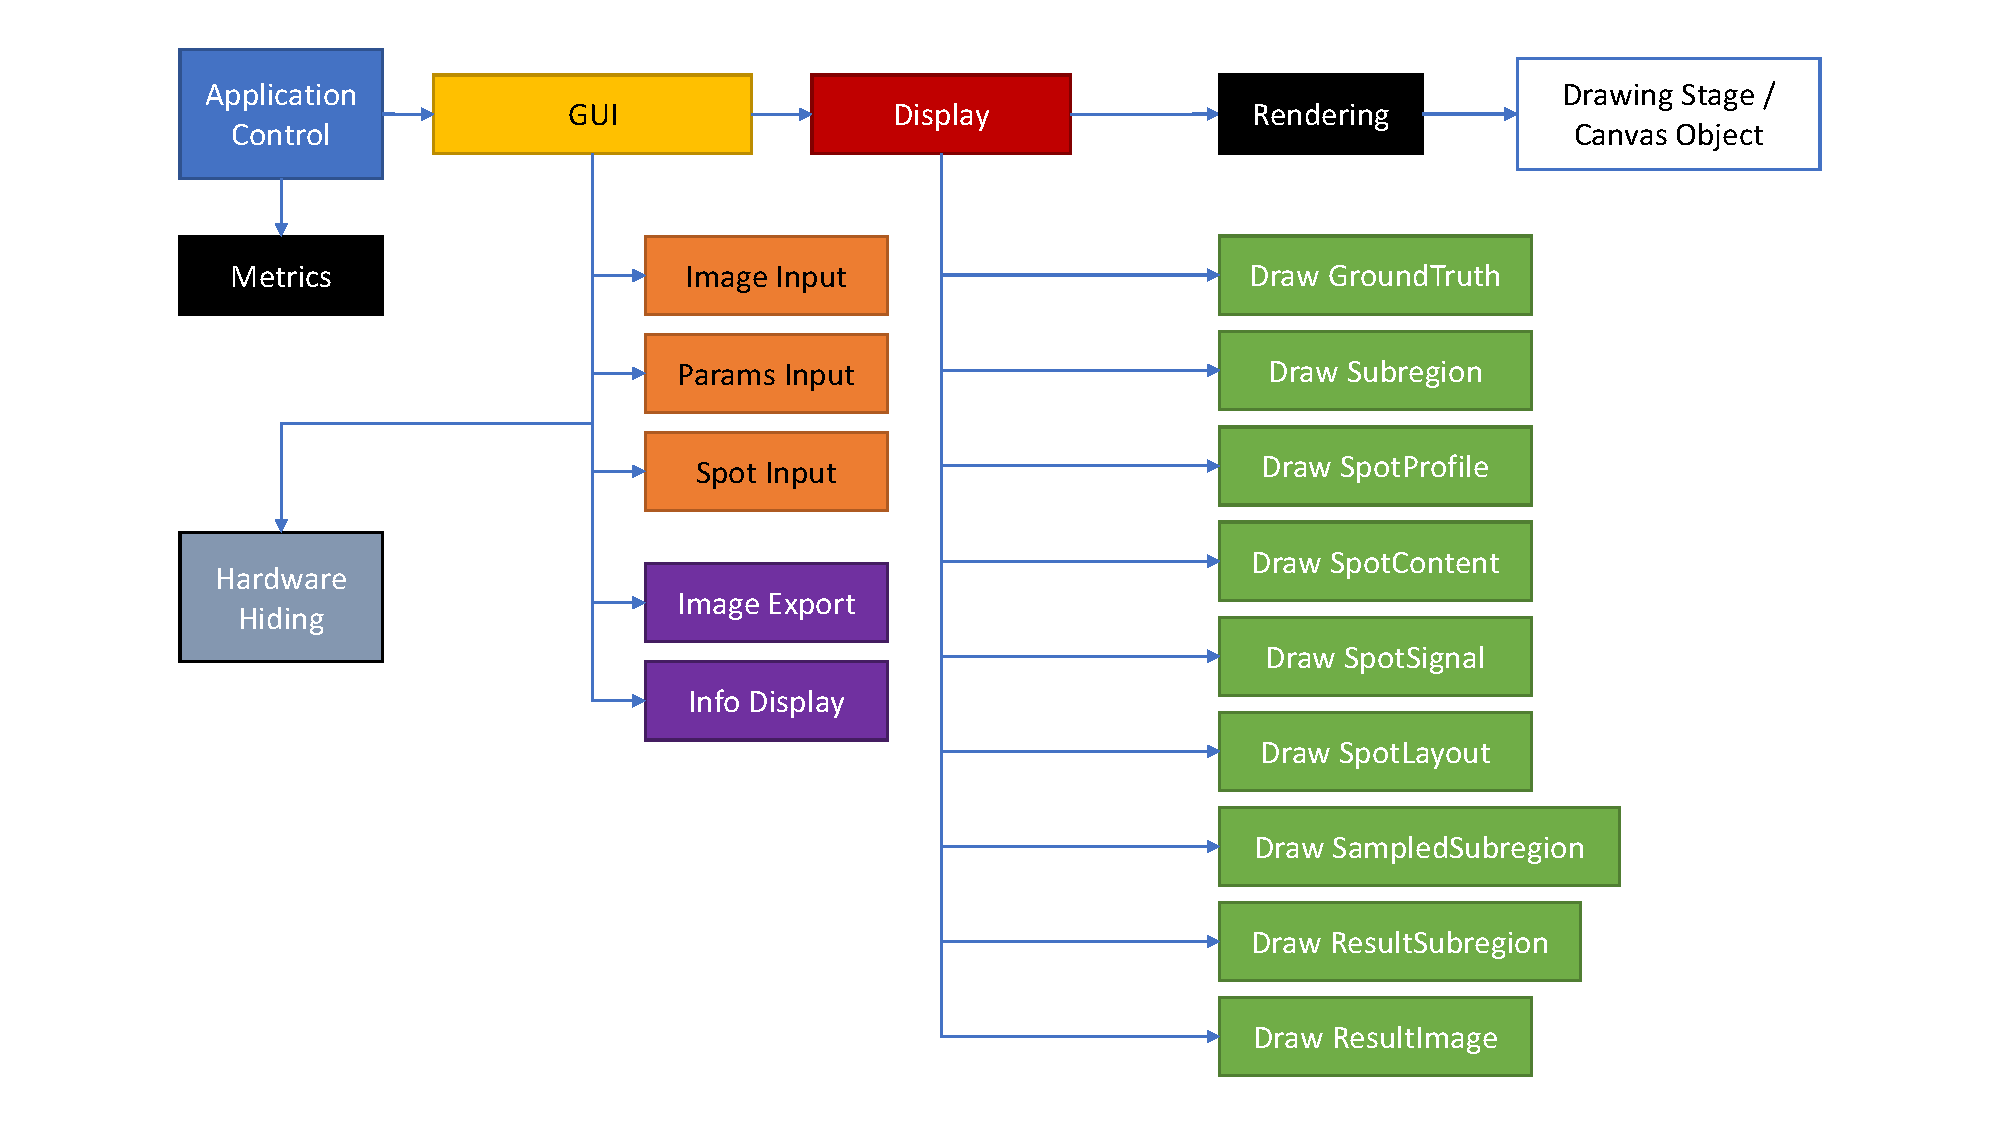
\includegraphics[width=1.00\textwidth]{MG_graph.pdf}
\caption{Use hierarchy among modules}
\label{FigUH}
\end{figure}

%\section*{References}

\bibliographystyle {plainnat}
\bibliography{../../../refs/References,../../../refs/cas741,../../../refs/programming}

\newpage{}

\end{document}